\documentclass{article}

\usepackage{graphicx}
\usepackage{tikz}
\usepackage{tikzsymbols}
\usetikzlibrary{calc,patterns,shapes.geometric}
\pagestyle{empty}
\usepackage[margin=0pt]{geometry}
\geometry{papersize={14in,12in}}

\def\centerarc[#1](#2)(#3:#4:#5){\draw[#1] ($(#2)+({#5*cos(#3)},{#5*sin(#3)})$) arc (#3:#4:#5);}

\begin{document}
	\begin{figure}
		\centering
		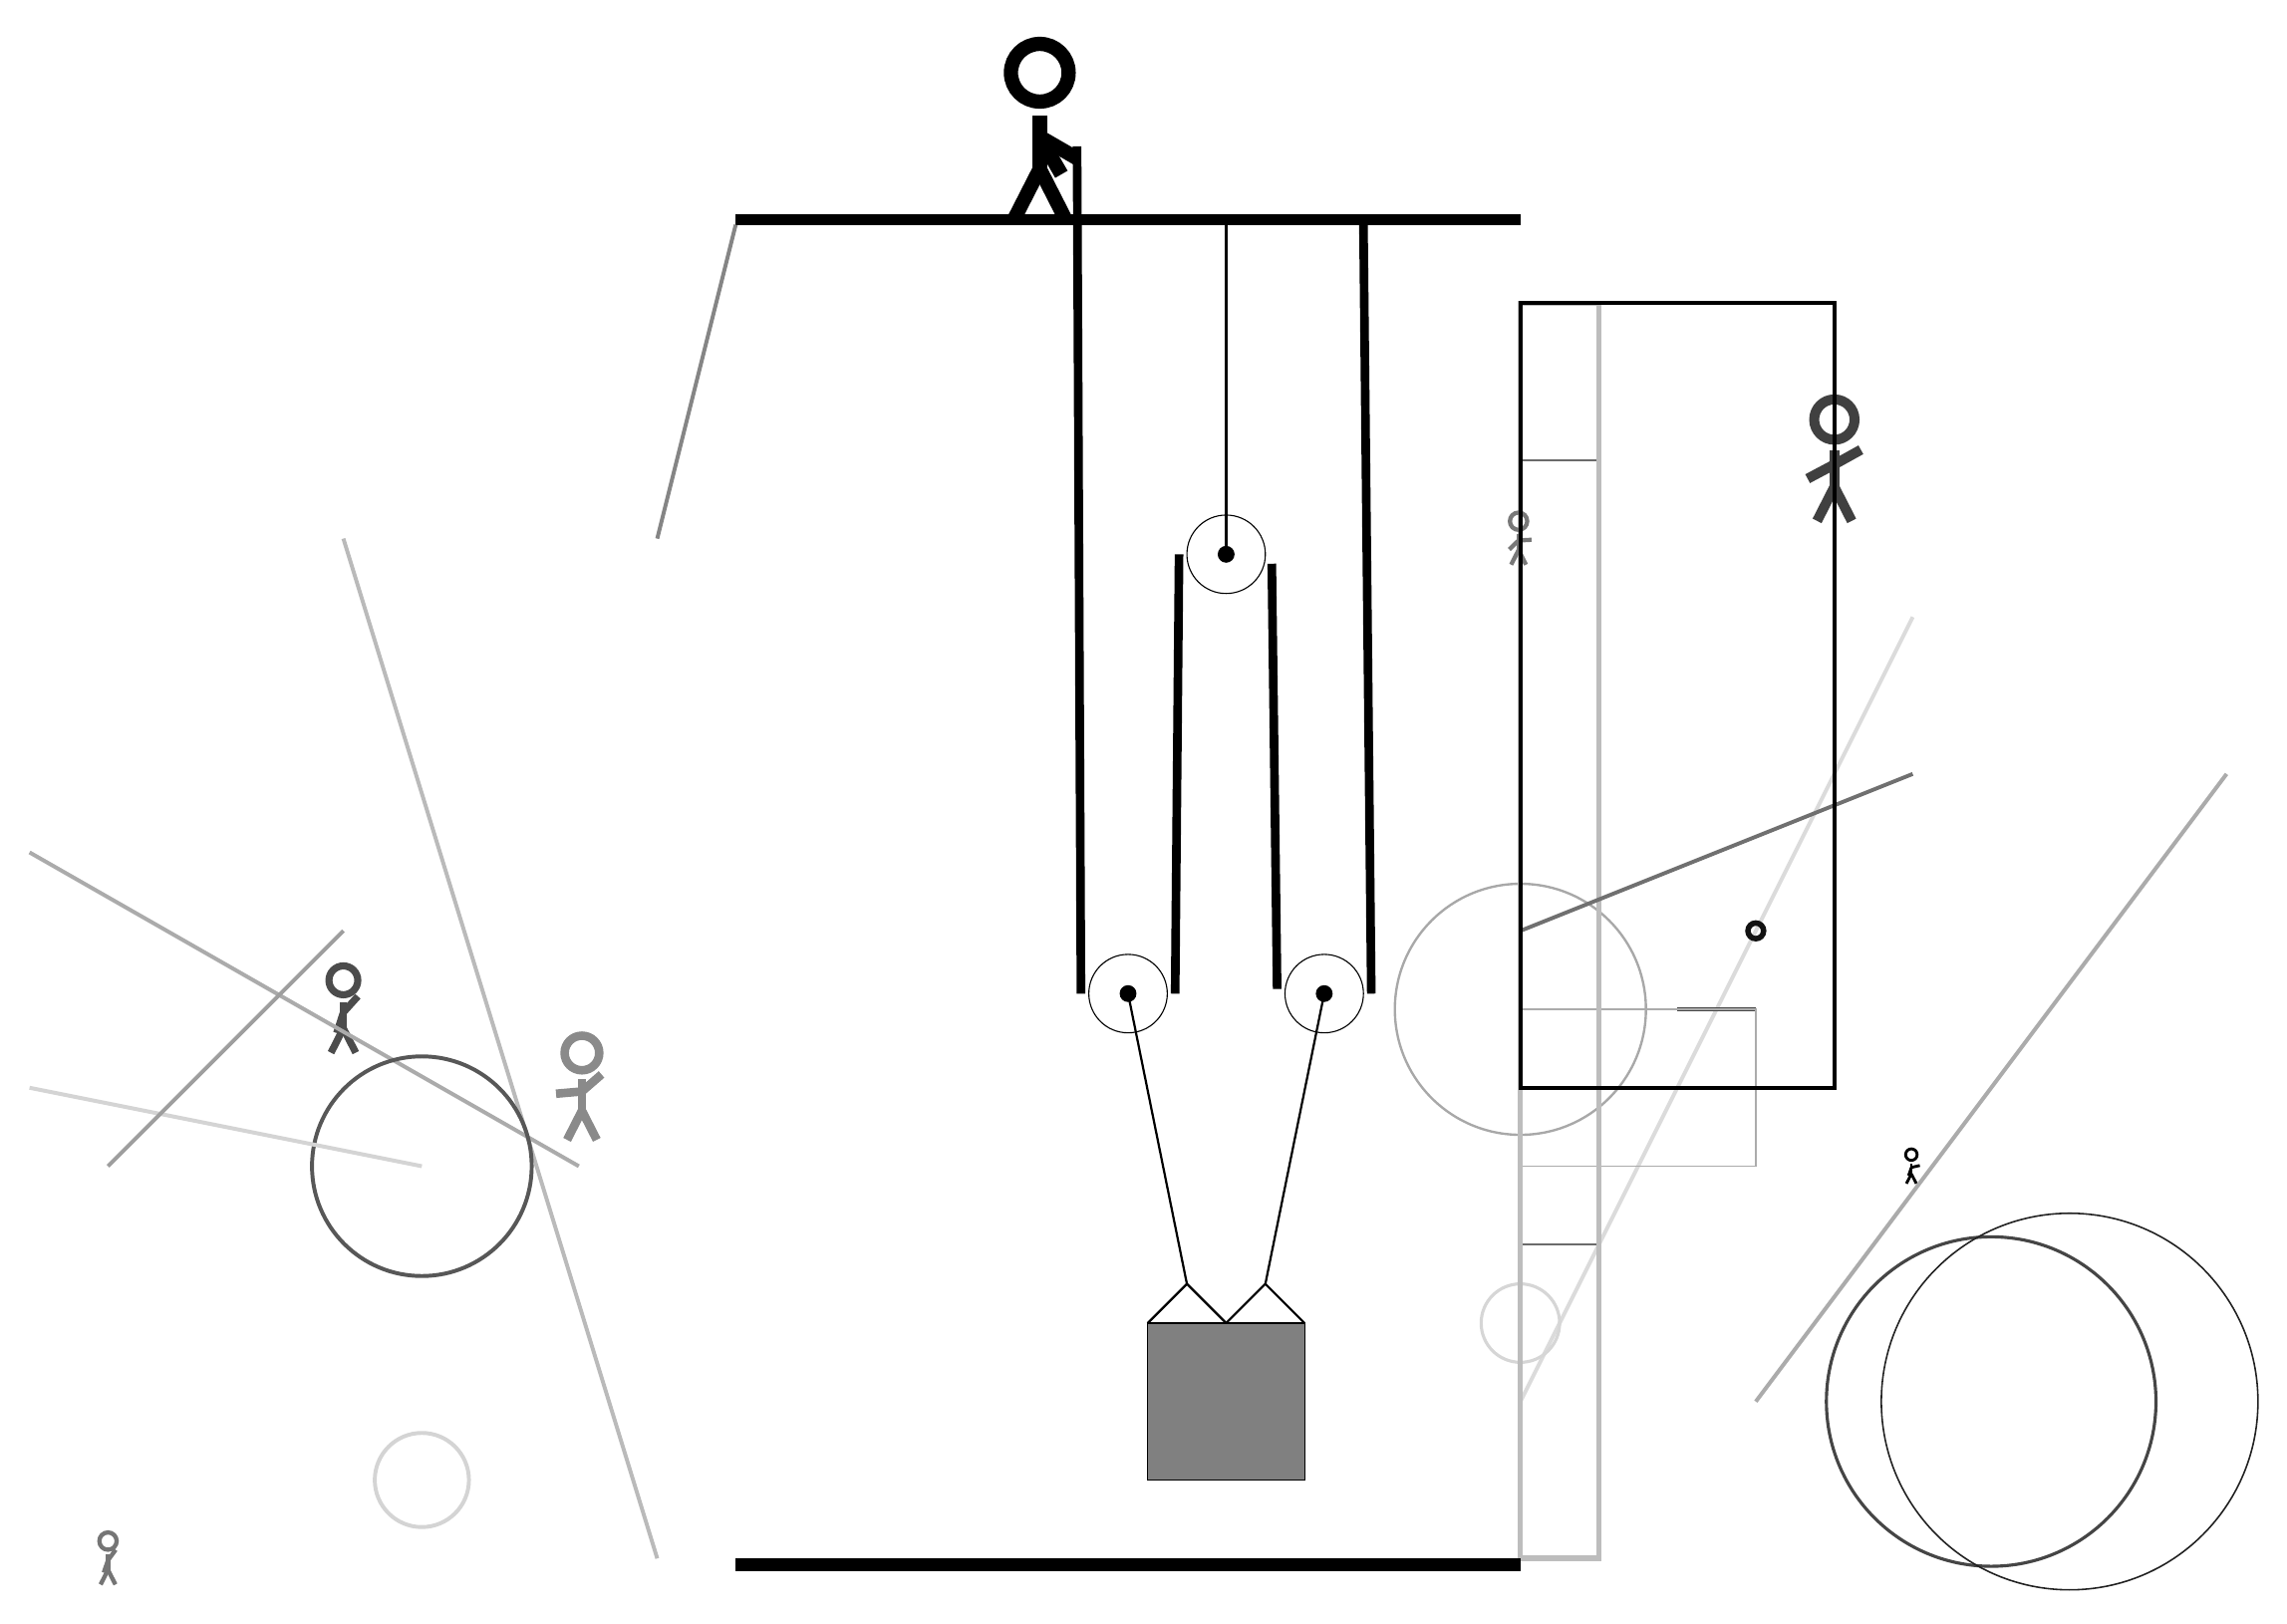
\begin{tikzpicture}
			%%%%% START %%%%%
			
			\draw[fill=black] (-4, 14) rectangle (6, 14.125);
			
			\draw (1, 4.2) circle (0.5);
			\draw[fill=black] (1, 4.2) circle (0.1);
			
			\draw (2.25, 9.8) circle (0.5);
			\draw[fill=black] (2.25, 9.8) circle (0.1);
			\draw[thick] (2.25, 9.8) -- (2.25, 14);
			
			\draw[line width=0.5mm, color=black!14](11, 9) -- (6, -1);
			
			\draw [line width=0.4mm, color=black!73](12, -1) circle (2.1);
			\draw[line width=0.6mm, color=black!72] (8, 4) rectangle (9, 4);
			\draw [line width=0.4mm, color=black!16](6, 0) circle (0.5);
			
			\draw [line width=0.3mm, color=black!34](6, 4) circle (1.6);
			\node[line width=0.5mm, color=black!70] at (-9, 4) {\Strichmaxerl[5][72][48]};
			
			\draw[line width=0.5mm, color=black!27](-9, 10) -- (-5, -3);
			
			\draw[line width=0.2mm, color=black!58] (7, 1) rectangle (6, 11);
			\node[line width=0.2mm, color=black!100] at (11, 2) {\Strichmaxerl[2][71][13]};
			\draw[line width=0.5mm, color=black!33](-6, 2) -- (-13, 6);
			
			\draw[line width=0.2mm, color=black!33] (6, 4) rectangle (9, 2);
			\draw [line width=0.5mm, color=black!66](-8, 2) circle (1.4);
			\draw[line width=0.7mm, color=black!26] (6, -3) rectangle (7, 13);
			\node[line width=0.2mm, color=black!53] at (6, 10) {\Strichmaxerl[3][44][3]};
			\node[line width=0.5mm, color=black!46] at (-6, 3) {\Strichmaxerl[6][5][41]};
			\draw [line width=0.5mm, color=black!17](-8, -2) circle (0.6);
			
			\node[line width=0.2mm, color=black!75] at (10, 11) {\Strichmaxerl[7][28][29]};
			\draw[line width=0.5mm, color=black!56](11, 7) -- (6, 5);
			\draw[line width=0.5mm, color=black!33](9, -1) -- (15, 7);
			\node[line width=0.4mm, color=black!54] at (-12, -3) {\Strichmaxerl[3][71][54]};
			\draw[line width=0.5mm, color=black!17](-8, 2) -- (-13, 3);
			
			\draw[line width=0.5mm, color=black!100] (6, 3) rectangle (10, 13);
			\draw [line width=0.2mm, color=black!87](13, -1) circle (2.4);
			\draw[line width=0.5mm, color=black!38](-9, 5) -- (-12, 2);
			\draw [line width=0.7mm, color=black!93](9, 5) circle (0.1);
			\draw[line width=0.5mm, color=black!48](-4, 14) -- (-5, 10);
			
			\draw (3.5, 4.2) circle (0.5);
			\draw[fill=black] (3.5, 4.2) circle (0.1);
			
			\draw[thick] (3.5, 4.2) -- (2.75, 0.5);
			\draw[thick] (1, 4.2) -- (1.75, 0.5);
			\draw[thick]  (1.25, 0) -- (1.75, 0.5) -- (2.25, 0);
			\draw[thick]  (2.25, 0) -- (2.75, 0.5) -- (3.25, 0);
			\draw[fill=black!50] (1.25, 0) rectangle (3.25, -2);
			
			\draw[line width=1.1mm] (0.35, 15) --  (0.4, 4.2);
			\centerarc[line width=1.1mm](1, 4.2)(180:360:0.6);
			\draw[line width=1.1mm] (1.6, 4.2) -- (1.65, 9.8);
			\centerarc[line width=1.1mm](2.25, 9.8)(-20:180:0.6);
			\draw[line width=1.1mm](2.832, 9.68) -- (2.9, 4.26);
			\centerarc[line width=1.1mm](3.5, 4.2)(160:360:0.6);
			\draw[line width=1.1mm](4.1, 4.2) -- (4.0, 14);
			
			\node at (-0.07, 15.2) {\Strichmaxerl[10][120][-30]};
			
			\draw[fill=black] (-4, -3) rectangle (6, -3.15);
			
			%%%%% END %%%%%
		\end{tikzpicture}
	\end{figure}	
\end{document}